\chapter{Οι Αλγόριθμοι}
\label{ch:Algorithms}

Σε αυτό το κεφάλαιο θα μελετήσουμε με λεπτομέρεια όλους τους αλγορίθμους που υλοποιήσαμε για τα AT-free γραφήματα.
Για κάθε αλγόριθμο θα δώσουμε τον συμβολισμό και τα λήμματα που χρειάζονται για την περιγραφή του. Αμέσως μετά, θα εξηγήσουμε την πολυπλοκότητά του και συγκεκριμένα βήματά του, που θεωρήσαμε πιο ιδιαίτερα. Τέλος θα δώσουμε και ένα απλό παράδειγμα επίλυσης του κάθε αλγορίθμου.

Διευκρινίζουμε ότι δεν αποδεικνύουμε την ορθότητα του κάθε αλγορίθμου που χρησιμοποιούμε. Οι αποδείξεις αυτές βρίσκονται στις αντίστοιχες αναφορές(\cite{at-free-independent-sets}, \cite{at-free-domination}, \cite{at-free-3-colouring})   

% -------------
% SECTION START
% -------------
\section{Υπολογισμός Μέγιστου Ανεξάρτητου Συνόλου}
\label{sec:Independent_Set_Alg}
Συμβολίζουμε τον αριθμό των κορυφών ενός γραφήματος $G = (V, E)$ με
$n$ και τον αριθμό των ακμών με $m$. 
Υπενθυμίζουμε ότι ένα ανεξάρτητο σύνολο σε ένα γράφημα $G$ είναι ένα σύνολο από ζεύγη με μη γειτονικές
κορυφές. Ο αριθμός ανεξαρτησίας ενός γραφήματος $G$, συμβολίζεται ως $\alpha(G)$ είναι το μέγεθος
του μεγαλύτερου ανεξάρτητου συνόλου στο γράφημα. Οι βασικές δομικές ιδιότητες που πρέπει να αναλύσουμε πριν την περιγραφή του αλγορίθμου είναι τα $Components$ και τα $Intervals$.


Σε ένα AT-free γράφημα $G$ όπου το $x$ και το $y$ είναι δύο ξεχωριστές μη γειτονικές κορυφές του G. Συμβολίζουμε με $C^{x}(y)$ το $Component$ του $G - N[x]$ όπου εμπεριέχεται το $y$, και με $r(x)$ τον αριθμό των $Components$ του $G - N[x]$.

\begin{definition}
	Μια κορυφή $z \in V \setminus \{x, y\}$ βρίσκεται μεταξύ των $x$ και $y$ εάν οι $x$ και $z$ βρίσκονται στο
	σε ένα $Component$ του$ G - N [y]$ και τα $y$ και $z$ βρίσκονται σε ένα $Component$ του $G - N [x]$.
\end{definition}

\begin{definition}
	Το διάστημα $I = I(x, y)$ του $G$ είναι το σύνολο όλων των κορυφών του $G$ που βρίσκονται μεταξύ $x$ και $y$. Συνεπώς, $I(x, y) = C_x(y) \cap C_y(x)$.
\end{definition}

Ο αλγόριθμος των Broersma, H., Kloks, T., Kratsch, D. και Müller, H. καθορίζει τον αριθμό ανεξαρτησίας κάθε $Component$ και κάθε $Interval$ χρησιμοποιώντας τις σχέσεις που δίνονται στα Λήμματα \ref{lemma6_1}, \ref{lemma6_2} και \ref{lemma6_3}.

\begin{lemma}
	\label{lemma6_1}
	Έστω ότι $G = (V,E)$ είναι οποιαδήποτε γράφημα. 
	Τότε $$\alpha(G)=1+\max_{x\in V}\left(\sum_{i=1}^{r(x)}\alpha(C_i^x)\right)$$ όπου  $C_1^x, C_2^x,...,C_{r(x)}^x$ τα $Compontes$ του $G - N[x]$.
\end{lemma}

\begin{lemma}
	\label{lemma6_2}
	Έστω ότι $G = (V,E)$ είναι ένα AT-free γράφημα. Έστω $x \in V$ και έστω $C^x$ ένα $Component$ του $G - N[x]$. Τότε $$\alpha(C^x)=1+\max_{y\in C^x}\left(\alpha(I(x,y))+\sum_{i}\alpha(D_i^y)\right)$$ όπου τα $D_i^y$ είναι $Components$ του $G - N[y]$ που εμπεριέχονται στο $C^x$. 
\end{lemma}

\begin{lemma}
	\label{lemma6_3}
	Έστω ότι $G = (V,E)$ είναι ένα AT-free γράφημα. Έστω $I = I(x,y)$ είναι ένα $Interval$ του $G$. Αν $I = \emptyset$ τότε $\alpha(I) = 0$. Αλλιώς $$\alpha(I)=1+\max_{s\in I}\left(\alpha(I(x,s))+\alpha(I(s,y))+\sum_{i}\alpha(C_i^s)\right)$$
\end{lemma}

Σε αυτό το σημείο μπορούμε να δώσουμε τον αλγόριθμο για τον υπολογισμό του αριθμού ανεξαρτησίας $\alpha(G)$ για AT-free γραφήματα, ο οποίος είναι βασισμένος στον δυναμικό προγραμματισμό. 

\begin{algorithm}[H]
	\caption{Αλγόριθμος υπολογισμού αριθμού ανεξαρτησίας σε AT-free γραφήματα}
	\label{alg:indep-set}
	
	\hspace*{\algorithmicindent} \textbf{Είσοδος:} Ένα AT-free γράφημα $G$.\\
	
	\hspace*{\algorithmicindent} \textbf{Έξοδος:} Αριθμός ανεξαρτησίας $\alpha(G)$
	
	\begin{algorithmic}[1]
		
		\STATE Για κάθε $x \in V$, υπολόγισε όλα τα $Components$ $C_1^x , C_2^x , \ldots , C_{r(x)}^x$
		\STATE Για κάθε ζευγάρι μη γειτονικών κορυφών $x$ και $y$, υπολόγισε το $Interval$ $I(x, y)$.
		\STATE Ταξινόμησε όλα τα $Components$ και τα $Intervals$ με βάση το μη-αύξοντα αριθμό κορυφών.
		\STATE Υπολόγισε τα $\alpha(C)$ και $\alpha(I)$ για κάθε $Components$ $C$ και κάθε $Interval$ $I$ με τη σειρά του Βήματος 3.
		\STATE Υπολόγισε το $\alpha(G)$.
		
	\end{algorithmic}
\end{algorithm}

\begin{definition}
	Υπάρχει αλγόριθμος χρόνου $O(n^4)$ για τον υπολογισμό του ανεξάρτητου αριθμού ενός AT-free γραφήματος.
\end{definition}

Για την πολυπλοκότητα του αλγορίθμου μελετάμε κάθε βήμα ξεχωριστά. Το πρώτο βήμα μπορεί να υλοποιηθεί σε χρόνο $O(n(n + m))$ χρησιμοποιώντας έναν γραμμικό αλγόριθμο για τον υπολογισμό των $Components$. 

Το βήμα 2 υπολογίζει $Intervals$ για τις μη γειτονικές κορυφές $x$ και $y$, χρησιμοποιώντας την τομή των συνιστωσών $C_x(y)$ και $C_y(x)$. Η διαδικασία, που εκτελείται σε χρόνο O(n) για κάθε $Interval$, οδηγεί σε συνολική χρονική πολυπλοκότητα $O(n^3)$. Η υλοποίηση αξιοποιεί ένα λεξικό με αντικείμενα της κλάσης $Interval$, παρέχοντας έναν αποτελεσματικό τρόπο διαχείρισης και υπολογισμού εντός το πολύ $n^2$ $Component$ και $Intervals$.

Με την χρήση του Bucket sort το βήμα 3 υλοποιείται σε $O(n^2)$.

Το σημείο φραγμού για τη χρονική πολυπλοκότητα του αλγορίθμου μας είναι το βήμα 4 αφού εκτελείται σε $O(n^4)$. Για κάθε $Component$ $C_x$ του $G - N[x]$ και μια κορυφή $y \in C_x$, ο αλγόριθμος πρέπει να υπολογίσει τα $Components$ του $G - N[y]$ που περιέχονται στην $C_x$. Αυτό γίνεται σε χρόνο $O(|C_x|)$ για σταθερές κορυφές $x$ και $y$ στο $C_x$, με αποτέλεσμα ο συνολικός χρόνος να είναι $O(n^3)$ για όλα τα $Compoents$. Θεωρώντας ένα $Interval$ $I(x, y)$ και μια κορυφή $s \in I$, ο αλγόριθμος πρέπει να αθροίσει τους αριθμούς ανεξαρτησίας των $Components$ $C_s$ του $G - N[s]$ που περιέχονται στο $I$. Η λειτουργία αυτή απαιτεί χρόνο $O(|I(x, y)|)$ για ένα σταθερό $I(x, y)$ και μια κορυφή $s \in I$. Ο συνολικός χρόνος για τον υπολογισμό του $\alpha(I)$ για όλα τα $Intervals$ είναι $O(n^3)$.

Είναι σαφές ότι το βήμα 5 μπορεί να γίνει σε χρόνο $O(n^2)$. Έτσι ο χρόνος εκτέλεσης του αλγορίθμου μας
είναι $O(n^4)$.

Ο αλγόριθμος έτσι όπως παρουσιάζεται από τους Broersma, H., Kloks, T., Kratsch, D. και Müller, H υπολογίζει τον αριθμό ανεξαρτησίας ενός AT-free γραφήματος. Έχουμε επεκτείνει την υλοποίηση του αλγορίθμου έτσι ώστε στο βήμα 5 ο αλγόριθμος να επιστρέφει και ένα μέγιστο ανεξάρτητο σύνολο. Ο τρόπος με τον οποίο το πετύχαμε αυτό είναι προσθέτοντας μια επιπλέον δομή αποθήκευσης, στην περίπτωση μας ένα λεξικό. Κάθε φόρα που υπολογίζαμε το μέγιστο alpha είτε για τα $Intervals$ \ref{lemma6_3}, είτε για τα $Components$ \ref{lemma6_2} αποθηκεύαμε στο λεξικό όλες τις ακμές από τα $Intervals$ και $Components$ που χρησιμοποιήθηκαν για να υπολογιστεί το μέγιστο alpha. Με αυτόν τον τρόπο στο τελευταίο βήμα είμαστε σε θέσει να επιστρέψουμε όλους τους κόμβους που χρειάστηκαν για τον υπολογισμό των alpha κάθε $Component$ του αθροίσματος \ref{lemma6_1} καθώς επίσης και το $x$ που αντιστοιχεί στο $1$ του τύπου.  

Παρακάτω παραθέτουμε ένα παράδειγμα εκτέλεσης του αλγορίθμου για το AT-free γράφημα \ref{fig:at-free-graph-example}.

\begin{figure}[H]
	\centering
	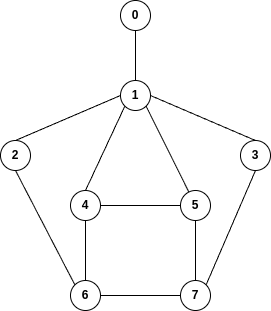
\includegraphics[width=0.4\textwidth]{pictures/at-free-graph.png} 
	\caption{Ένα AT-free γράφημα με 8 κόμβους}
	\label{fig:at-free-graph-example}
\end{figure}

Μετά την εκτέλεση του πρώτου βήματος τα $Components$ που υπολογίσαμε φαίνονται στον πίνακα \ref{table:first-step-intependent-set} 

% Components
\begin{table}[H]
	
	\centering
	\caption{Components του γραφήματος μετά την εκτέλεση του πρώτου βήματος}
	\begin{tabular}{|c|c|c|}
		\hline
		\textbf{Component} & \textbf{Σύνολο κορυφών} & \textbf{Alpha} \\
		\hline
		$C_1^1$ & \quad \{6, 7\} & - \\
		$C_1^4$ & \quad \{2, 6\} & - \\
		$C_2^4$ & \quad \{0\} & - \\
		$C_3^4$ & \quad \{5\} & - \\
		$C_1^3$ & \quad \{2\} & - \\
		$C_2^3$ & \quad \{7, 5\} & - \\
		$C_3^3$ & \quad \{0\} & - \\
		$C_1^2$ & \quad \{3, 4, 5, 7\} & - \\
		$C_2^2$ & \quad \{0\} & - \\
		$C_1^0$ & \quad \{4, 3, 2, 6, 7, 5\} & - \\
		$C_1^6$ & \quad \{1, 4, 0, 5\} & - \\
		$C_1^7$ & \quad \{1, 3, 2, 0\} & - \\
		$C_1^5$ & \quad \{3, 4, 6, 2\} & - \\
		$C_2^5$ & \quad \{0\} & - \\		
		\hline
	\end{tabular}
	\label{table:first-step-intependent-set}
\end{table}

Για το δεύτερο βήμα του αλγορίθμου, παίρνοντας όλους τους συνδυασμούς μη γειτονικών κορυφών για το παρών γράφημα. Τα $Intervals$ που προκύπτουν φαίνονται στον παρακάτω πίνακα\ref{table:second-step-intependent-set}. 

\begin{table}[H]
	
	\centering
	\caption{Intervals του γραφήματος μετά την εκτέλεση του δεύτερου βήματος}
	\begin{tabular}{|c|c|c|}
		\hline
		\textbf{Intervals} & \textbf{Σύνολο κορυφών} & \textbf{Alpha} \\
		\hline
		I(2, 5) & \quad \{3, 4\} & - \\
		I(2, 7) & \quad \{3\} & - \\
		I(5, 2) & \quad \{3, 4\} & - \\
		I(5, 6) & \quad \{4\} & - \\
		I(0, 7) & \quad \{2, 3\} & - \\
		I(0, 6) & \quad \{4, 5\} & - \\
		I(7, 2) & \quad \{3\} & - \\
		I(7, 0) & \quad \{2, 3\} & - \\
		I(6, 5) & \quad \{4\} & - \\
		I(6, 0) & \quad \{4, 5\} & - \\
		\hline
	\end{tabular}
	\label{table:second-step-intependent-set}
\end{table}

Όπως φαίνεται και στους πίνακες \ref{table:sorted-components} και \ref{table:sorted-intervals},μετά το τρίτο βήμα τα $Components$ και $Intervals$ ταξινομούνται με βάση το πλήθος των κορυφών τους, από το μικρότερο στο μεγαλύτερο.

\begin{table}[H]
	\centering
	\caption{Ταξινόμηση Components με βάση το σύνολο κορυφών}
	\begin{tabular}{|c|c|c|}
		\hline
		\textbf{Components} & \textbf{Σύνολο Κορυφών} & \textbf{Alpha} \\
		\hline
		$C_2^4$ & \quad \{0\} & - \\
		$C_3^4$ & \quad \{5\} & - \\
		$C_1^3$ & \quad \{2\} & - \\
		$C_3^3$ & \quad \{0\} & - \\
		$C_2^2$ & \quad \{0\} & - \\
		$C_2^5$ & \quad \{0\} & - \\
		$C_1^1$ & \quad \{6, 7\} & - \\
		$C_1^4$ & \quad \{2, 6\} & - \\
		$C_2^3$ & \quad \{7, 5\} & - \\
		$C_1^2$ & \quad \{3, 4, 5, 7\} & - \\
		$C_1^6$ & \quad \{1, 4, 0, 5\} & - \\
		$C_1^7$ & \quad \{1, 3, 2, 0\} & - \\
		$C_1^5$ & \quad \{3, 4, 6, 2\} & - \\
		$C_1^0$ & \quad \{4, 3, 2, 6, 7, 5\} & - \\
		\hline
	\end{tabular}
	\label{table:sorted-components}
\end{table} 

\begin{table}[H]
	\centering
	\caption{Ταξινόμηση Intervals με βάση το σύνολο κορυφών}
	\begin{tabular}{|c|c|c|}
		\hline
		\textbf{Intervals} & \textbf{Σύνολο Κορυφών} & \textbf{Alpha} \\
		\hline
		I(2, 7) & \{3\} & - \\
		I(5, 6) & \{4\} & - \\
		I(7, 2) & \{3\} & - \\
		I(6, 5) & \{4\} & - \\
		I(2, 5) & \{3, 4\} & - \\
		I(5, 2) & \{3, 4\} & - \\
		I(0, 7) & \{2, 3\} & - \\
		I(0, 6) & \{4, 5\} & - \\
		I(7, 0) & \{2, 3\} & - \\
		I(6, 0) & \{4, 5\} & - \\
		\hline
	\end{tabular}
	\label{table:sorted-intervals}
\end{table}

Χρησιμοποιώντας τα λήμματα \ref{lemma6_1}, \ref{lemma6_2} και εφαρμόζοντας τεχνικές δυναμικού προγραμματισμού, μετά την εκτέλεση του βήματος τέσσερα έχουν υπολογιστεί τα alpha όλων των $Components$ και $Intervals$. Τα αποτελέσματα φαίνονται στους πίνακες \ref{table:computed-alpha-componentes}  και \ref{table:computed-alpha-intervals}

\begin{table}[H]
	\centering
	\caption{Πίνακας Components μετά την εκτέλεση του βήματος 4 του αλγορίθμου}
	\begin{tabular}{|c|c|c|}
		\hline
		\textbf{Components} & \textbf{Σύνολο Κορυφών} & \textbf{Alpha} \\
		\hline
		$C_2^4$ & \quad \{0\} & 1 \\
		$C_3^4$ & \quad \{5\} & 1 \\
		$C_1^3$ & \quad \{2\} & 1 \\
		$C_3^3$ & \quad \{0\} & 1 \\
		$C_2^2$ & \quad \{0\} & 1 \\
		$C_2^5$ & \quad \{0\} & 1 \\
		$C_1^1$ & \quad \{6, 7\} & 1 \\
		$C_1^4$ & \quad \{2, 6\} & 1 \\
		$C_2^3$ & \quad \{7, 5\} & 1 \\
		$C_1^2$ & \quad \{3, 4, 5, 7\} & 2 \\
		$C_1^6$ & \quad \{1, 4, 0, 5\} & 3 \\
		$C_1^7$ & \quad \{1, 3, 2, 0\} & 3 \\
		$C_1^5$ & \quad \{3, 4, 6, 2\} & 2 \\
		$C_1^0$ & \quad \{4, 3, 2, 6, 7, 5\} & 3 \\
		\hline
	\end{tabular}
	\label{table:computed-alpha-componentes}
\end{table} 

\begin{table}[H]
	\centering
	\caption{Πίνακας Intervals μετά την εκτέλεση του βήματος 4 του αλγορίθμου}
	\begin{tabular}{|c|c|c|}
		\hline
		\textbf{Intervals} & \textbf{Σύνολο Κορυφών} & \textbf{Alpha} \\
		\hline
		I(2, 7) & \{3\} & 1 \\
		I(5, 6) & \{4\} & 1 \\
		I(7, 2) & \{3\} & 1 \\
		I(6, 5) & \{4\} & 1 \\
		I(2, 5) & \{3, 4\} & 1 \\
		I(5, 2) & \{3, 4\} & 1 \\
		I(0, 7) & \{2, 3\} & 2 \\
		I(0, 6) & \{4, 5\} & 2 \\
		I(7, 0) & \{2, 3\} & 2 \\
		I(6, 0) & \{4, 5\} & 2 \\
		\hline
	\end{tabular}
	\label{table:computed-alpha-intervals}
\end{table}

Στο τελευταίο βήμα με την εφαρμογή του λήμματος \ref{lemma6_1}, είναι προφανές ότι ο αριθμός ανεξαρτησίας για το παρόν γράφημα είναι τέσσερα. Αυτό μπορεί, στο συγκεκριμένο παράδειγμα, να προκύψει από διάφορες κορυφές. Στο παρακάτω  σχήμα φαίνεται ένα μέγιστο ανεξάρτητο σύνολο που έχει προκύψει από τον κόμβο $4$.

\begin{figure}[H]
	\centering
	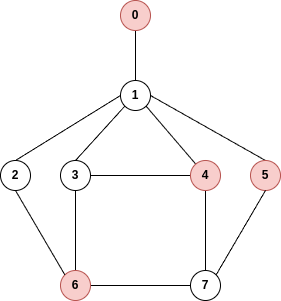
\includegraphics[width=0.4\textwidth]{pictures/at-free-graph.intependent-set.png} 
	\caption{Μέγιστο Ανεξάρτητο Σύνολο σε AT-free γράφημα}
	\label{fig:at-free-graph-independent-set}
\end{figure}


\section{Υπολογισμός Ελάχιστου Κυρίαρχου Συνόλου}
\label{sec:Domination_Set_Alg}

Θα αναλύσουμε πεπερασμένα, μη-κατευθυνόμενα γραφήματα. Έστω $G = (V, E)$ ένα γράφημα. Ορίζουμε \( n \) ως τον αριθμό των κορυφών του \( G \) και \( G[W] \) ως το υπογράφημα που επάγεται από το \( W \subseteq V \). Η γειτονιά \( N(v) = \{w  \in V : \{v,w\} \in E\} \) αποτελείται από τις κορυφές που συνδέονται με το \( v \in V \). Το \( N[v] = N(v) \cup \{v\} \) είναι η κλειστή γειτονιά του \( u \in V \), ενώ το \( N[W] = \bigcup_{w \in W} N[w] \) αποτελεί την γειτονιά που εκτείνεται από το \( W \).

Μια ακολουθία κορυφών ενός γραφήματος \( G=(V, E) \) αποτελεί ένα μονοπάτι \( P=(u=x_0,x_1,\dots, x_k =u) \) στο \( G \), όπου \( \{x_i, x_{i+1}\} \in E \) για κάθε \( i \in \{0, 1, \dots,k-1\} \). Το μήκος \( k \) είναι η απόσταση ενός μονοπατιού \( P =(u=x_0, x_1, \dots, x_k=u) \).

Η απόσταση μεταξύ δύο κορυφών \( u \) και \( v \) στο \( G \), συμβολίζεται ως \( d_G (u,v) \) και ορίζεται ως το ελάχιστο μήκος ενός μονοπατιού μεταξύ των \( u \) και \( v \). Η διάμετρος ενός γραφήματος \( G \) ορίζεται ως \( diam(G) = \max \{d_G(u,v): u,v \in V \} \).

Ένα υποσύνολο \( D \subseteq V \) είναι ένα κυρίαρχο σύνολο του \( G = (V,E) \) αν για κάθε κορυφή \( u \in V \setminus D \) υπάρχει μια κορυφή \( v \in D \) τέτοια ώστε \( \{u, v\} \in E \), δηλαδή \( N[D] = V \). Συμβολίζουμε το ελάχιστο κυρίαρχο σύνολο ενός γραφήματος \( G \) με \( \gamma(G) \).

\begin{definition}
	Ένα μονοπάτι $P = (x_0, x_1,\dots , x_d =y)$ είναι ένα κυρίαρχο συντομότερο μονοπάτι (DSP εν συντομία) ενός γραφήματος $G=(V,E)$, αν $dG(x,y) = d$ και ${x_0, x_1, \dots , x_d}$ είναι ένα κυριάρχο σύνολο του $G$.
\end{definition}

\begin{theorem}
	\label{domination-set-dsp-theorem}
	Έστω $G = (V,E)$ ένα γράφημα με DSP $P =(x=x_0,x_1, \dots , x_d=y)$.  Έστω $H_0 ={x},H_1 = N(x),\dots ,H_i = {w \in V: D_G(x,w) = i}, \dots,H_l = {w \in V: d_G(x,w)=l}$
	είναι τα BFS-επίπεδα του $x$. Τότε υπάρχει ένα ελάχιστης πληθικότητας κυρίαρχο σύνολο $D$ του $G$ τέτοιο ώστε
\end{theorem}

\begin{center}
	\[
	\displaystyle \LARGE  \bigwedge_{i\in\{0,1,\ldots,\ell\}} \bigwedge_{j\in\{0,1,\ldots,\ell-i\}} \left|D\cap\bigcup_{s=i}^{i+j}H_{s}\right| \leq j+4
	\]
\end{center}

\begin{theorem}
	\label{domination-set-main-definiton}
	Έστω $G = (V,E)$ ένα συνδεδεμένο γράφημα χωρίς $AT$. Υπάρχει μια κορυφή $x\in V$
	που μπορεί να προσδιοριστεί σε γραμμικό χρόνο με την ακόλουθη ιδιότητα. Έστω $H_0,H_1,\dots , H_l$
	είναι τα BFS-επίπεδα του $x$. Τότε υπάρχει ένα ελάχιστης πληθικότητας κυρίαρχο σύνολο $D$ του $G$ τέτοιο ώστε
\end{theorem}

\begin{center}
	\[
	\displaystyle \LARGE  \bigwedge_{i\in\{0,1,\ldots,\ell\}} \bigwedge_{j\in\{0,1,\ldots,\ell-i\}} \left|D\cap\bigcup_{s=i}^{i+j}H_{s}\right| \leq j+3
	\]
\end{center}

Η βασική ιδέα του αλγορίθμου μας είναι ο υπολογισμός ενός κυρίαρχου συνόλου μέσω δυναμικού προγραμματισμού με τη χρήση των επιπέδων ενός δέντρου BFS. Ας εξετάσουμε ορισμένες λεπτομέρειες. Για εμάς, μια υποεπίλυση είναι ένα σύνολο $\mathbf{S}\subseteq\bigcup_{j=0}^{i-1}H_{j}$, που επιλέγεται κατά τη διάρκεια του δυναμικού προγραμματισμού μέχρι ένα σταθερό επίπεδο \( i - 1 \in \{1, 2, \dots ,l-1\} \). Για να συλλέξουμε τις σχετικές πληροφορίες οποιασδήποτε υποεπίλυσης \( S \), επιλέγουμε να αποθηκεύσουμε το υποσύνολο των κορυφών των υπολύσεων που ανήκουν στα δύο τελευταία επίπεδα, δηλαδή \( S \cap (H_{i-2} \cup H_{i-1}) \). Το άνω όριο για τον μέγιστο αριθμό κορυφών ενός ελάχιστου κυρίαρχου συνόλου που μπορεί να έχει σε οποιαδήποτε τρία διαδοχικά επίπεδα BFS είναι ζωτικής σημασίας για τον χρόνο εκτέλεσης του αλγορίθμου. Έχουμε δείξει ότι αυτός ο αριθμός είναι το πολύ 6 για γραφήματα με DSP \ref{domination-set-dsp-theorem}  και το πολύ 5 για συνδεδεμένα γραφήματα χωρίς \(AT\) \ref{domination-set-main-definiton}.


Θα παρουσιάσουμε τον αλγόριθμο $mcds_w(G)$, όπου $w$ είναι ένας σταθερός θετικός ακέραιος, που υπολογίζει ένα κυρίαρχο σύνολο για ένα συνδεδεμένο γράφημα $G$. Αυτός ο αλγόριθμος θα μπορούσε να εφαρμοστεί και σε γενικά γραφήματα ως ένας απλός ευρετικός αλγόριθμος. Ωστόσο, η συμπεριφορά αυτού του αλγορίθμου μπορεί να είναι πολύ κακή. Για παράδειγμα, εάν, για όλα τα κυρίαρχα σύνολα $D$ γραφήματος εισόδου $G = (V, E)$ και για όλες τις κορυφές $x$ του $G$, υπάρχουν τρία διαδοχικά επίπεδα BFS του $x$ έτσι ώστε το $S$ να έχει περισσότερες από $w$ κορυφές σε αυτά τα τρία επίπεδα, τότε η έξοδος του $mcds_w(G)$ είναι απλώς το τετριμμένο κυρίαρχο σύνολο $V$. Εάν το γράφημα εισόδου G έχει μια κορυφή x και ένα κυρίαρχο σύνολο ελάχιστης πληθικότητας $D$ έτσι ώστε το πολύ $w$ κορυφές του $D$ να ανήκουν σε οποιαδήποτε τρία διαδοχικά επίπεδα BFS, τότε η $mcds_w(G)$ εξάγει ένα ελάχιστο κυρίαρχο σύνολο του $G$.


\begin{algorithm}[H]
	\caption{Αλγόριθμος υπολογισμού ελάχιστου κυρίαρχου συνόλου σε AT-free γραφήματα $mcds_w$}
	\label{alg:domi-set}
	\hspace*{\algorithmicindent} \textbf{Είσοδος:} Ένα AT-free γράφημα $G = (V,E)$.\\
	\hspace*{\algorithmicindent} \textbf{Έξοδος:} Ελάχιστο κυρίαρχο σύνολο $D \subseteq V$
	
	\begin{algorithmic}[1]	
		\STATE Αρχικοποίησε το $D := V$;
		\FOR{όλα τα $x \in V$}
		\STATE Υπολόγισε τα επίπεδα BFS του κόμβου $x$:
		\STATE $H_0 = \{x\}$; $H_1 = N(x)$; $\ldots$; $H_l = \{u \in V : d_G(x, u) = l\}$;
		\STATE $i := 1$;
		\STATE Αρχικοποίησε την ουρά $A_1$ ώστε να περιέχει μια διατεταγμένη τριάδα $(S, S, \text{val}(S))$ για όλα τα μη κενά υποσύνολα $S$ του $N[x]$ που ικανοποιούν το $\text{val}(S) := |S| \leq w$;
		\WHILE{$A_i \neq \emptyset$ \textbf{and} $i < l$}
		\STATE $i := i + 1$;
		\FOR{όλες τις τριάδες $(S, S', \text{val}(S'))$ στην ουρά $A_{i-1}$}
		\FOR{κάθε $U \subseteq H_i$ με $|S \cup U| \leq w$}
		\IF{$N[S \cup U] \supseteq H_{i-1}$}
		\STATE $R := (S \cup U) \setminus H_{i-2}$;
		\STATE $R' := S' \cup U$;
		\STATE $\text{val}(R') := \text{val}(S') + |U|$;
		\IF{δεν υπάρχει καμία τριάδα στην $A_i$ με πρώτη εγγραφή $R$}
		\STATE πρόσθεσε το $(R, R', \text{val}(R'))$ στην ουρά $A_i$;
		\ENDIF
		\IF{υπάρχει μια τριάδα $(P, P', \text{val}(P'))$ in $A_i$ όπου $P = R$ and $\text{val}(R') < \text{val}(P')$}
		\STATE αντικατέστησε το $(P, P', \text{val}(P'))$ μέσα στην $A_i$ με $(R, R', \text{val}(R'))$;
		\ENDIF
		\ENDIF
		\ENDFOR
		\ENDFOR
		\ENDWHILE
		\STATE Μεταξύ όλων των τριάδων $(S, S', \text{val}(S'))$ στην ουρά $A_l$ που ικανοποιούν $H_l \subseteq N[S]$, προσδιορίστε μία με ελάχιστη τιμή $\text{val}(S')$, έστω $(B, B', \text{val}(B'))$;
		\IF{$\text{val}(B') < |D|$}
		\STATE $D := B'$;
		\ENDIF
		\ENDFOR
	\end{algorithmic}
	
\end{algorithm}

\begin{theorem}
	Ο αλγόριθμος $mcds_w(G)$ υπολογίζει σε χρόνο $O(n^{w+2})$ ένα ελάχιστo κυρίαρχο σύνολο ενός συνδεδεμένου γραφήματος $G= (V,E)$ αν το $G$ έχει ελάχιστο 
	κυρίαρχο σύνολο $D$ και μια κορυφή $x\in V$ έτσι ώστε το πολύ $w$ κορυφές του $D$ να ανήκουν
	σε οποιαδήποτε τρία διαδοχικά επίπεδα BFS του $x$.
\end{theorem}

\begin{theorem}
	\label{domi-set-theomrem-5}
	Υπάρχει ένας αλγόριθμος χρόνου $O(n^7)$ για τον υπολογισμό ενός ελάχιστου κυρίαρχου συνόλου οποιουδήποτε γραφήματος για το οποίο κάθε συνδεδεμένη συνιστώσα έχει ένα κυρίαρχο συντομότερο μονοπάτι.
\end{theorem}
Κατ' αναλογία, τα θεωρήματα \ref{domination-set-main-definiton} και \ref{domi-set-theomrem-5} υποδηλώνουν ότι ο αλγόριθμος $mcds_5(G)$ υπολογίζει για ένα δοθέν
συνδεδεμένο γράφημα AT-free ένα ελάχιστο κυρίαρχο σύνολο. Επιπλέον, αρκεί να υπολογίσουμε ένα κυρίαρχο ζεύγος $(x,y)$ και στη συνέχεια να ελέγξουμε τα επίπεδα BFS
της κορυφής x μόνο. Έτσι, λαμβάνουμε

\begin{theorem}
	Υπάρχει ένας αλγόριθμος χρόνου $O(n^6)$ για τον υπολογισμό ελάχιστου
	κυρίαρχου συνόλου για οποιοδήποτε δεδομένο γράφημα χωρίς ΑΤ.
\end{theorem}

Παρακάτω παραθέτουμε ένα παράδειγμα εκτέλεσης του αλγορίθμου για τον κόμβο 1 του AT-free γραφήματος \ref{fig:at-free-graph-example-domi}.

\begin{figure}[H]
	\centering
	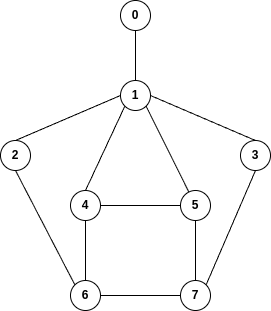
\includegraphics[width=0.4\textwidth]{pictures/at-free-graph.png} 
	\caption{Ένα AT-free γράφημα με 8 κόμβους}
	\label{fig:at-free-graph-example-domi}
\end{figure}


\begin{table}[H]
	\centering
	\caption{Επίπεδα BFS του κόμβου 1}
	\label{tab:bfs_levels}
	\begin{tabular}{|c|l|}
		\hline
		\textbf{Επίπεδα} & \textbf{Κορυφές} \\
		\hline
		0 & $\{1\}$ \\
		1 & $\{0, 2, 3, 4, 5\}$ \\
		2 & $\{6, 7\}$ \\
		\hline
	\end{tabular}
\end{table}

\begin{longtable}{|c|c|c|}
	\caption{Αρχικοποίηση Ουράς $\text{Α}_{\text{1}}$} \\
	\hline
	\textbf{S} & \textbf{S'} & \textbf{val(S)} \\
	\hline
	\endfirsthead % Header for first page
	\hline
	\textbf{S} & \textbf{S'} & \textbf{val(S)} \\
	\hline
	\endhead % Header for subsequent pages
	$\{4\}$ & $\{4\}$ & 1 \\
	$\{3\}$ & $\{3\}$ & 1 \\
	$\{2\}$ & $\{2\}$ & 1 \\
	$\{0\}$ & $\{0\}$ & 1 \\
	$\{5\}$ & $\{5\}$ & 1 \\
	$\{1\}$ & $\{1\}$ & 1 \\
	$\{4,3\}$ & $\{4,3\}$ & 2 \\
	$\{4,2\}$ & $\{4,2\}$ & 2 \\
	$\{4,0\}$ & $\{4,0\}$ & 2 \\
	$\{4,5\}$ & $\{4,5\}$ & 2 \\
	$\{4,1\}$ & $\{4,1\}$ & 2 \\
	$\{3,2\}$ & $\{3,2\}$ & 2 \\
	$\{3,0\}$ & $\{3,0\}$ & 2 \\
	$\{3,5\}$ & $\{3,5\}$ & 2 \\
	$\{3,1\}$ & $\{3,1\}$ & 2 \\
	$\{2,0\}$ & $\{2,0\}$ & 2 \\
	$\{5,2\}$ & $\{5,2\}$ & 2 \\
	$\{2,1\}$ & $\{2,1\}$ & 2 \\
	$\{5,0\}$ & $\{5,0\}$ & 2 \\
	$\{1,0\}$ & $\{1,0\}$ & 2 \\
	$\{5,1\}$ & $\{5,1\}$ & 2 \\
	$\{4,3,2\}$ & $\{4,3,2\}$ & 3 \\
	$\{4,3,0\}$ & $\{4,3,0\}$ & 3 \\
	$\{4,3,5\}$ & $\{4,3,5\}$ & 3 \\
	$\{4,3,1\}$ & $\{4,3,1\}$ & 3 \\
	$\{4,2,0\}$ & $\{4,2,0\}$ & 3 \\
	$\{4,5,2\}$ & $\{4,5,2\}$ & 3 \\
	$\{4,2,1\}$ & $\{4,2,1\}$ & 3 \\
	$\{4,5,0\}$ & $\{4,5,0\}$ & 3 \\
	$\{4,1,0\}$ & $\{4,1,0\}$ & 3 \\
	$\{4,5,1\}$ & $\{4,5,1\}$ & 3 \\
	$\{3,2,0\}$ & $\{3,2,0\}$ & 3 \\
	$\{5,3,2\}$ & $\{5,3,2\}$ & 3 \\
	$\{3,2,1\}$ & $\{3,2,1\}$ & 3 \\
	$\{3,5,0\}$ & $\{3,5,0\}$ & 3 \\
	$\{3,1,0\}$ & $\{3,1,0\}$ & 3 \\
	$\{3,5,1\}$ & $\{3,5,1\}$ & 3 \\
	$\{5,2,0\}$ & $\{5,2,0\}$ & 3 \\
	$\{2,1,0\}$ & $\{2,1,0\}$ & 3 \\
	$\{5,2,1\}$ & $\{5,2,1\}$ & 3 \\
	$\{5,1,0\}$ & $\{5,1,0\}$ & 3 \\
	$\{4,3,2,0\}$ & $\{4,3,2,0\}$ & 4 \\
	$\{4,3,2,5\}$ & $\{4,3,2,5\}$ & 4 \\
	$\{4,3,2,1\}$ & $\{4,3,2,1\}$ & 4 \\
	$\{4,3,5,0\}$ & $\{4,3,5,0\}$ & 4 \\
	$\{4,3,1,0\}$ & $\{4,3,1,0\}$ & 4 \\
	$\{4,3,5,1\}$ & $\{4,3,5,1\}$ & 4 \\
	$\{4,5,2,0\}$ & $\{4,5,2,0\}$ & 4 \\
	$\{4,2,1,0\}$ & $\{4,2,1,0\}$ & 4 \\
	$\{4,5,2,1\}$ & $\{4,5,2,1\}$ & 4 \\
	$\{4,5,1,0\}$ & $\{4,5,1,0\}$ & 4 \\
	$\{5,3,2,0\}$ & $\{5,3,2,0\}$ & 4 \\
	$\{3,2,1,0\}$ & $\{3,2,1,0\}$ & 4 \\
	$\{5,3,2,1\}$ & $\{5,3,2,1\}$ & 4 \\
	$\{3,5,1,0\}$ & $\{3,5,1,0\}$ & 4 \\
	$\{5,2,1,0\}$ & $\{5,2,1,0\}$ & 4 \\
	$\{4,2,5,3,0\}$ & $\{4,2,5,3,0\}$ & 5 \\
	$\{4,2,3,0,1\}$ & $\{4,2,3,0,1\}$ & 5 \\
	$\{4,2,5,3,1\}$ & $\{4,2,5,3,1\}$ & 5 \\
	$\{4,5,3,0,1\}$ & $\{4,5,3,0,1\}$ & 5 \\
	$\{4,2,5,0,1\}$ & $\{4,2,5,0,1\}$ & 5 \\
	$\{2,5,3,0,1\}$ & $\{2,5,3,0,1\}$ & 5 \\
	\hline
	\label{tab:A1-domi}
\end{longtable}

\begin{longtable}{|c|c|c|}
	\caption{Ουρά $\text{Α}_{\text{l}}$ μετά την εκτέλεση του δυναμικού αλγορίθμου} \\
	\hline
	\textbf{S} & \textbf{S'} & \textbf{val(S)} \\
	\hline
	\endfirsthead % Header for first page
	\hline
	\textbf{S} & \textbf{S'} & \textbf{val(S)} \\
	\hline
	\endhead % Header for subsequent pages
	$\{6,7,0\}$ & $\{7,6,0\}$ & 3 \\
	$\{6\}$ & $\{6,1\}$ & 2 \\
	$\{7\}$ & $\{7,1\}$ & 2 \\
	$\{6,7\}$ & $\{7,6,1\}$ & 3 \\
	$\{4,6,7,0\}$ & $\{4,7,6,0\}$ & 4 \\
	$\{4,6\}$ & $\{4,6,1\}$ & 3 \\
	$\{4,7\}$ & $\{4,7,1\}$ & 3 \\
	$\{4,6,7\}$ & $\{4,7,6,1\}$ & 4 \\
	$\{6,3,7,0\}$ & $\{7,3,6,0\}$ & 4 \\
	$\{3,6\}$ & $\{3,6,1\}$ & 3 \\
	$\{3,7\}$ & $\{3,7,1\}$ & 3 \\
	$\{6,3,7\}$ & $\{7,3,6,1\}$ & 4 \\
	$\{6,2,7,0\}$ & $\{7,2,6,0\}$ & 4 \\
	$\{2,6\}$ & $\{2,6,1\}$ & 3 \\
	$\{2,7\}$ & $\{2,7,1\}$ & 3 \\
	$\{6,2,7\}$ & $\{7,2,6,1\}$ & 4 \\
	$\{6,5,7,0\}$ & $\{7,5,6,0\}$ & 4 \\
	$\{6,0\}$ & $\{1,6,0\}$ & 3 \\
	$\{7,0\}$ & $\{1,7,0\}$ & 3 \\
	$\{5,6\}$ & $\{5,6,1\}$ & 3 \\
	$\{5,7\}$ & $\{5,7,1\}$ & 3 \\
	$\{6,5,7\}$ & $\{7,5,6,1\}$ & 4 \\
	$\{4,6,3,7,0\}$ & $\{4,3,6,0,7\}$ & 5 \\
	$\{4,3,6\}$ & $\{4,3,6,1\}$ & 4 \\
	$\{4,3,7\}$ & $\{4,3,7,1\}$ & 4 \\
	$\{4,3,6,7\}$ & $\{4,3,6,7,1\}$ & 5 \\
	$\{4,2,7,0\}$ & $\{4,2,7,0\}$ & 4 \\
	$\{4,2,6,7,0\}$ & $\{4,2,6,0,7\}$ & 5 \\
	$\{4,2,6\}$ & $\{4,2,6,1\}$ & 4 \\
	$\{4,2,7\}$ & $\{4,2,7,1\}$ & 4 \\
	$\{4,2,6,7\}$ & $\{4,2,6,7,1\}$ & 5 \\
	$\{4,5,6,0\}$ & $\{4,5,6,0\}$ & 4 \\
	$\{4,6,5,7,0\}$ & $\{4,6,0,7,5\}$ & 5 \\
	$\{4,6,0\}$ & $\{4,1,6,0\}$ & 4 \\
	$\{4,7,0\}$ & $\{4,1,7,0\}$ & 4 \\
	$\{4,5,6\}$ & $\{4,5,6,1\}$ & 4 \\
	$\{4,5,7\}$ & $\{4,5,7,1\}$ & 4 \\
	$\{4,5,6,7\}$ & $\{4,6,7,5,1\}$ & 5 \\
	$\{3,2,7,0\}$ & $\{3,2,7,0\}$ & 4 \\
	$\{2,6,3,7,0\}$ & $\{3,2,6,0,7\}$ & 5 \\
	$\{3,2,6\}$ & $\{3,2,6,1\}$ & 4 \\
	$\{3,2,7\}$ & $\{3,2,7,1\}$ & 4 \\
	$\{3,2,6,7\}$ & $\{3,2,6,7,1\}$ & 5 \\
	$\{3,5,6,0\}$ & $\{3,5,6,0\}$ & 4 \\
	$\{6,5,3,7,0\}$ & $\{3,6,0,7,5\}$ & 5 \\
	$\{3,6,0\}$ & $\{3,1,6,0\}$ & 4 \\
	$\{3,7,0\}$ & $\{3,1,7,0\}$ & 4 \\
	$\{3,5,6\}$ & $\{3,5,6,1\}$ & 4 \\
	$\{3,5,7\}$ & $\{3,5,7,1\}$ & 4 \\
	$\{3,5,6,7\}$ & $\{3,6,7,5,1\}$ & 5 \\
	$\{2,6,5,7,0\}$ & $\{2,6,0,7,5\}$ & 5 \\
	$\{2,6,0\}$ & $\{2,1,6,0\}$ & 4 \\
	$\{2,7,0\}$ & $\{2,1,7,0\}$ & 4 \\
	$\{5,2,6\}$ & $\{5,2,6,1\}$ & 4 \\
	$\{5,2,7\}$ & $\{5,2,7,1\}$ & 4 \\
	$\{5,2,6,7\}$ & $\{2,6,7,5,1\}$ & 5 \\
	$\{5,6,0\}$ & $\{5,1,6,0\}$ & 4 \\
	$\{5,7,0\}$ & $\{5,1,7,0\}$ & 4 \\
	$\{4,2,3,7,0\}$ & $\{4,3,2,7,0\}$ & 5 \\
	$\{4,3,2,6\}$ & $\{4,3,2,6,1\}$ & 5 \\
	$\{4,3,2,7\}$ & $\{4,3,2,7,1\}$ & 5 \\
	$\{4,6,5,3,0\}$ & $\{4,3,6,0,5\}$ & 5 \\
	$\{4,3,6,0\}$ & $\{4,3,6,0,1\}$ & 5 \\
	$\{4,3,7,0\}$ & $\{4,3,7,0,1\}$ & 5 \\
	$\{4,3,5,6\}$ & $\{4,3,6,5,1\}$ & 5 \\
	$\{4,3,5,7\}$ & $\{4,3,7,5,1\}$ & 5 \\
	$\{4,2,6,5,0\}$ & $\{4,2,6,0,5\}$ & 5 \\
	$\{4,2,5,7,0\}$ & $\{4,2,7,0,5\}$ & 5 \\
	$\{4,2,6,0\}$ & $\{4,2,6,0,1\}$ & 5 \\
	$\{4,5,2,6\}$ & $\{4,2,6,5,1\}$ & 5 \\
	$\{4,5,2,7\}$ & $\{4,2,7,5,1\}$ & 5 \\
	$\{4,5,7,0\}$ & $\{4,7,0,5,1\}$ & 5 \\
	$\{2,6,5,3,0\}$ & $\{3,2,6,0,5\}$ & 5 \\
	$\{2,5,3,7,0\}$ & $\{3,2,7,0,5\}$ & 5 \\
	$\{3,2,6,0\}$ & $\{3,2,6,0,1\}$ & 5 \\
	$\{5,3,2,6\}$ & $\{3,2,6,5,1\}$ & 5 \\
	$\{5,3,2,7\}$ & $\{3,2,7,5,1\}$ & 5 \\
	$\{3,5,7,0\}$ & $\{3,7,0,5,1\}$ & 5 \\
	$\{5,2,6,0\}$ & $\{2,6,0,5,1\}$ & 5 \\
	$\{5,2,7,0\}$ & $\{2,7,0,5,1\}$ & 5 \\
	\hline
	\label{tab:Al-domi}
\end{longtable}


Από τη γραμμή 25 του αλγορίθμου \ref{alg:domi-set} προκύπτει ότι η τετράδα με το ελάχιστο $val(S')$ είναι η $(\{6\}, \{6, 1\}, 2)$, αφού ισχύει και η συνθήκη $H_l \subseteq N[S]$ ($\{6,7\} \subseteq \{6,2,7,3\}$). Άρα, το ελάχιστο κυρίαρχο σύνολο είναι το $\{6, 1\}$.

\begin{figure}[H]
	\centering
	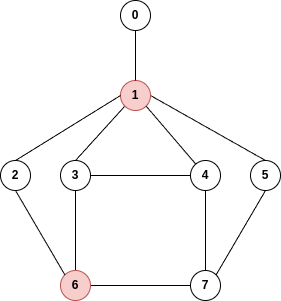
\includegraphics[width=0.4\textwidth]{pictures/at-free-graph-domi-set.png} 
	\caption{Ελάχιστο Κυρίαρχο Σύνολο σε AT-free γράφημα}
	\label{fig:at-free-graph-domi-set}
\end{figure}

% SECTION START
% -------------
\section{Το Πρόβλημα του 3-Χρωματισμού}
\label{sec:3-Coloring_Alg}


Για το Πρόβλημα του 3-Χρωματισμού θεωρούμε ότι ένα γράφημα είναι πάντα απλό, μη κατευθυνόμενο και χωρίς βρόχους. Για μια κορυφή $v$ ενός γραφήματος $G$, συμβολίζουμε με $N_G(v)$ το σύνολο των κορυφών που είναι γειτονικές με την $v$ στο $G$ και γράφουμε $N_G[v] = N_G(v) \cup \{v\}$. Αποσύρουμε τον δείκτη $G$ και γράφουμε $N(v)$ και $N[v]$ όποτε αυτό είναι σαφές από τα συμφραζόμενα. Για $X \subseteq V(G)$, γράφουμε $G[X]$ για το υπογράφημα του $G$ που επάγεται από το $X$, και γράφουμε $G - X$ για το υπογράφημα του $G$ που επάγεται από το $V(G) \setminus X$. Ένα σύνολο $X \subseteq V(G)$ είναι σταθερό αν το $G[X]$ δεν περιέχει ακμές. Το $K_n$ δηλώνει το πλήρες γράφημα (δηλαδή το γράφημα με όλες τις πιθανές ακμές) σε $n$ κορυφές, και το διαμάντι είναι το (μοναδικό) γράφημα με $4$ κορυφές με $5$ ακμές \ref{fig:diamond-k4}.

\begin{figure}[H]
	\centering
	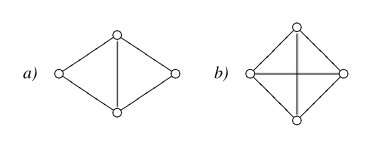
\includegraphics[width=0.4\textwidth]{pictures/diamond-k4.png} 
	\caption{(\textbf{α}) Διαμάντι, (\textbf{β}) $\text{Κ}_{\text{4}}$}
	\label{fig:diamond-k4}
\end{figure}

Γράφουμε $G/S$ για το γράφημα που λαμβάνουμε από το $G$ με τη σύμπτυξη όλων των
κορυφών του S σε μία μόνο κορυφή. Δηλαδή,

$V(G/s)=\left(V(G)\setminus S\right)\cup\{s\}\quad\mathrm{where}\ s\notin V(G),$

$E(G/s)=\left\{x y\in E(G)\mid x,y\notin S\right\}\cup\left\{s y\mid x y\in E(G)\land x\in S\land y\notin S\right\}$


Ένα σύνολο $S \subseteq V(G)$ αποσυνδέει τις κορυφές $a$ και $b$ στο $G$ αν $a$ και $b$ ανήκουν σε διαφορετικές συνδεδεμένες συνιστώσες του $G - S$. Ορίζουμε το $S$ ως σύνολο αποκοπής του $G$ αν αποσυνδέει ορισμένες κορυφές $a$ και $b$. Επιπλέον, το $S$ ονομάζεται ελάχιστο διαχωριστικό (\textit{minimal separator}) του $G$ αν υπάρχουν κορυφές $a$ και $b$ τέτοιες ώστε το $S$ να αποσυνδέει τις $a$ και $b$, αλλά κανένα υποσύνολο του $S$ να μην μπορεί να τις αποσυνδέσει. Ένα σημείο αποκοπής (\textit{cutpoint}) του $G$ είναι μια κορυφή $v$ τέτοια ώστε το σύνολο $\{v\}$ να λειτουργεί ως σύνολο αποκοπής. Ένα μπλοκ του $G$ είναι ένα μέγιστο συνδεδεμένο επαγόμενο
υπογράφημα του $G$ που δεν έχει σημεία αποκοπής.

Παρουσιάζουμε τα απαραίτητα Θεωρήματα και Λήμματα για την υλοποίηση του αλγορίθμου.

\begin{theorem}
	\label{theor:1.1}
	Υπάρχει ένας αλγόριθμος χρόνου $O(n^2m)$ για να αποφασίσουμε, δεδομένου ενός AT-free γραφήματος
	G με $n$ κορυφές και $m$ ακμές, αν το $G$ είναι ή όχι 3-χρωματίσιμο και να κατασκευάσει επίσης
	ένα 3-χρωματισμό $G$, αν υπάρχει.
\end{theorem}

\begin{theorem}
	\label{theor:1.2}
	Έστω $G$ ένα γράφημα AT-free με τουλάχιστον τρεις κόμβους και χωρίς κανένα επαγόμενο διαμάντι ή $K_4$.
	\begin{enumerate}
		\item $G$ είναι τριγωνική λωρίδα (\textit{triangular strip}) \ref{fig:triangular-strip}, ή
		\item $G$ περιέχει ένα σταθερό cutset.
	\end{enumerate}
\end{theorem}


\begin{figure}[H]
	\centering
	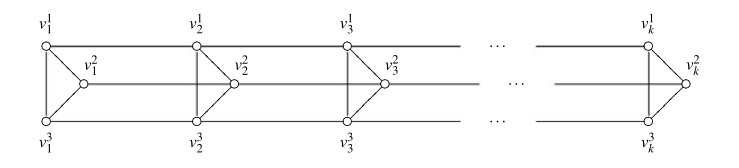
\includegraphics[width=0.8\textwidth]{pictures/triangular-strip.png} 
	\caption{Tριγωνική Λωρίδα (\textit{triangular strip}) τάξης k}
	\label{fig:triangular-strip}
\end{figure}

\begin{theorem}
	\label{theor:1.3}
	Κάθε γράφημα $G$ που είναι AT-free και δεν περιέχει επαγόμενο διαμάντι και $K_4$ είναι 3-χρωματίσιμο. Επιπλέον, αν το $G$ περιέχει ένα ελάχιστο σταθερό διαχωριστικό $S$, τότε υπάρχει ένας 3-χρωματισμός του $G$ στον οποίο όλοι οι κόμβοι του $S$ έχουν τον ίδιο χρωματισμό.
\end{theorem}

\begin{theorem}
	\label{theor:3.1}
	Αν οι κόμβοι $u, v$ είναι γειτονικοί σε ένα γράφημα $G$ που είναι AT-free και $S$ είναι ένα μέγιστο σταθερό σύνολο στο $N(u) \cap N(v)$, τότε το $G/S$ είναι AT-free. Επιπλέον, το $G$ είναι 3-χρωματίσιμο αν και μόνο αν το $G/S$ είναι.
\end{theorem}


\begin{lemma}
	\label{lemma:3.4}
	Αν το $G$ είναι AT-free και το $S$ είναι ένα ελάχιστο διαχωριστικό σύνολο, τότε το $G/S$ είναι επίσης AT-free.
\end{lemma}

\begin{lemma}
	\label{lemma:4.1}
	Έστω $G$ ένα ισχυρά συνεκτικό γράφημα γράφημα AT-free χωρίς επαγόμενο διαμάντι και $K_4$. Τότε κάθε κόμβος του $G$ βρίσκεται το πολύ σε ένα τρίγωνο.
\end{lemma}

\begin{lemma}
	\label{lemma:6.1}
	Αν το $S$ είναι ένα ελάχιστο σταθερό διαχωριστικό ενός γραφήματος $G$ που είναι AT-free, τότε υπάρχει ένας κόμβος $x \in V(G)$ με $N(x) \supseteq S$.
\end{lemma}


\begin{lemma}
	\label{lemma:6.2}
	Αν το $S$ είναι ένα σταθερό διαχωριστικό ενός συνεκτικού γραφήματος $G$, και $S \subseteq S$ είναι ένα σταθερό σύνολο, τότε το $S$ είναι επίσης ένα σταθερό διαχωριστικό του $G$.
\end{lemma}


\begin{lemma}
	\label{lemma:6.3}
	Ένα σύνολο $S \subseteq V(G)$ είναι ένα ελάχιστο διαχωριστικό ενός γραφήματος $G$ με $|S| \geq 2$ αν και μόνο αν υπάρχει ένα μπλοκ $B$ του $G$ τέτοιο ώστε το $S$ να είναι ένα ελάχιστο διαχωριστικό του $B$.
\end{lemma}


Για την απόδειξη του Θεωρήματος \ref{theor:1.1} πρέπει:
\begin{enumerate}
	\item Μειώσουμε το πρόβλημα σε γραφήματα AT-free χωρίς επαγόμενα διαμάντια,
	\item Αα αποσυνθέσουμε κάθε AT-free γράφημα χωρίς επαγόμενα διαμάντια και χωρίς $K_4$ σε τριγωνικές λωρίδες χρησιμοποιώντας σταθερά διαχωριστικά, και
	\item Να συμπτύξουμε ελάχιστα σταθερά διαχωριστικά χωρίς να αλλάξουμε την απάντηση στο πρόβλημα.
\end{enumerate}

Αυτό μειώνει το πρόβλημα σε γραφήματα τα οποία κάθε μπλοκ είναι μια τριγωνική λωρίδα ή έχει το πολύ δύο κόμβους. Σε αυτά τα γραφήματα είναι εύκολο να κατασκευάσουμε τον 3-χρωματισμό τους. Αν σε οποιοδήποτε στάδιο συναντήσουμε ένα $K_4$, δηλώνουμε ότι ο γράφημα δεν είναι $3$-χρωματίσιμο.

Παρουσιάζουμε ένα περίγραμμα αλγορίθμου που προκύπτει από αυτό που έχουμε αναφέρει:
\begin{algorithm}[H]
	\caption{Αλγόριθμος επίλυσης του προβλήματος 3-χρωματισμού για AT-free γραφήματα}
	\label{alg:coloring}
	
	\hspace*{\algorithmicindent} \textbf{Είσοδος:} Ένα AT-free γράφημα $G$.\\
	
	\hspace*{\algorithmicindent} \textbf{Έξοδος:} Ένα 3-χρωματισμό του $G$ ή "Το $G$ δεν είναι 3-χρωματίσιμο".
	
	\begin{algorithmic}[1]
		
		\IF{το $G$ περιέχει ένα $\text{Κ}_{\text{4}}$}
		\STATE \textbf{return} "Το $G$ δεν είναι 3-χρωματίσιμο"
		\ENDIF
		\STATE /* Τώρα το $G$ δεν περιέχει $\text{Κ}_{\text{4}}$ */
		\IF{το $G$ περιέχει γειτονικές κορυφές $u$, $v$ με $|N(u) \cap N(v)| \geq 2$}
		\STATE \textbf{return} Αναδρομικά βρες τον 3-χρωματισμό του $G/N(u) \cap N(v)$
		\ENDIF
		\STATE /* Τώρα το $G$ δεν περιέχει επαγόμενα διαμάντια και κανένα $\text{Κ}_{\text{4}}$ */
		\IF{το $G$ περιέχει έναν ελάχιστο σταθερό διαχωριστή $S$ με $|S| \geq 2$}
		\STATE \textbf{return} Αναδρομικά βρες τον 3-χρωματισμό του $G/S$
		\ENDIF
		\STATE /* Τώρα κάθε τμήμα του $G$ είναι είτε τριγωνική λωρίδα είτε έχει το πολύ 2 κορυφές */
		\STATE \textbf{return} Κατασκεύασε τον 3-χρωματισμό του $G$
	\end{algorithmic}
\end{algorithm}

Η χρονική πολυπλοκότητα του παρόν αλγορίθμου είναι $O(n^2m)$. Για να το αποδείξουμε αυτό αρκεί να δείξουμε πώς μπορούμε να υλοποιήσουμε τις γραμμές 1,5,9 και 13 του αλγορίθμου.

Για την γραμμή 1 του αλγορίθμου η διαδικασία έχει ως εξής: Εάν η γραμμή 1 εκτελείται για πρώτη φορά, ελέγχουμε εάν το γράφημα $G$ περιέχει ένα πλήρες γράφημα με τέσσερις κορυφές ($K_4$) σε χρόνο πολυπλοκότητας $O(m^2) = O(n^2 \cdot m)$ εξετάζοντας όλα τα πιθανά ζεύγη μη συνδεδεμένων ακμών στο $G$. Εάν η γραμμή 1 επιτυγχάνεται μέσω αναδρομής στο $G/S$, όπου $s$ είναι η κορυφή του $G/S$ που προκύπτει από τη σύμπτυξη του $S$, τότε χρειάζεται μόνο να ελέγξουμε εάν η γειτονιά του $s$ στο $G/S$ περιέχει ένα τρίγωνο. Αυτός ο έλεγχος μπορεί να γίνει σε χρόνο $O(n \cdot m)$ εξετάζοντας κάθε ζεύγος κορυφής-ακμής του $G$. Αρκεί για να επαληθεύσουμε ότι το $G/S$ δεν περιέχει ένα $K_4$, καθώς πριν από τη σύμπτυξη του $S$, το γράφημα $G$ θεωρήσαμε ότι δεν περιέχει $K_4$ (φτάσαμε τουλάχιστον στη γραμμή 5 πριν από την αναδρομική κλήση).

Η διαδικασία ελέγχου για την γραμμή 5 υλοποιείται με πολυπλοκότητα $O(nm)$. Διατρέχουμε κάθε ακμή $uv$ του $G$ και κατασκευάζουμε την τομή των γειτονιών των $u$ και $v$, που συμβολίζεται ως $N(u) \cap N(v)$, εξερευνώντας τις γειτονιές των $u$ και $v$ ξεχωριστά. Αυτή η εξερεύνηση γίνεται σε χρόνο $O(n)$ για κάθε κορυφή, με αποτέλεσμα η συνολική χρονική πολυπλοκότητα να είναι $O(nm)$.

Για να υλοποιήσουμε τον έλεγχο στη γραμμή 9 με χρονική πολυπλοκότητα $O(nm)$, χρησιμοποιούμε το Λήμμα \ref{lemma:6.3}, το οποίο δηλώνει ότι ο έλεγχος κάθε μπλοκ $B$ του $G$ για έναν ελάχιστο σταθερό διαχωριστή είναι επαρκής. Σύμφωνα με το Λήμμα \ref{lemma:6.1}, αν υπάρχει ένας τέτοιος διαχωριστής $S$ του $B$, είναι επίσης ένα σταθερό cutset του $B$, υπονοώντας την ύπαρξη μιας κορυφής $x$ με $N_B(x)$ που περιέχει το $S$. Με $|V(B)| \geq 3$ και $|S| \geq 2$, όπως προκύπτει από το Λήμμα \ref{lemma:6.3}, το $B$ είναι ισχυρά συνεκτικό γράφημα και δεν περιέχει κανένα διαμάντι ή $K_4$, όντας ένας επαγόμενο υπογράφα του $G$. Επομένως, το $N_B(x)$ περιέχει το πολύ δύο μέγιστα σταθερά σύνολα, εκ των οποίων το ένα περιέχει το $S$, καθορίζοντας το ως σταθερό cutset του $B$ από το Λήμμα \ref{lemma:6.2}.

Για να προχωρήσουμε, υπολογίζουμε πρώτα τα μπλοκ που προκύπτουν από τον αλγόριθμο "Biconnectivity" του Robert Tarjan \cite{tarjan-depth-first-search} στο $G$ σε χρόνο $O(n + m)$. Στη συνέχεια, επαναλαμβάνουμε για κάθε κορυφή $x$ στο $V(G)$ και κάθε μπλοκ $B$ του $G$ που περιέχει το $x$ με τουλάχιστον τρεις κορυφές. Για κάθε τέτοιο συνδυασμό, ελέγχουμε αν το $N_B(x)$, το $N_B(x) \setminus \{u\}$, ή το $N_B(x) \setminus \{v\}$ είναι ένα σταθερό cutset του $B$, όπου $uv$ (αν υπάρχει) είναι η μοναδική ακμή στο $G[N_B(x)]$. Αυτή η δοκιμή μπορεί να ολοκληρωθεί σε χρόνο $O(|V(B)| + |E(B)|)$ χρησιμοποιώντας τον αλγόριθμο αναζήτησης "Depth-first search". Δεδομένου ότι $|V(B)| \leq |E(B)|$ για κάθε μπλοκ $B$ του $G$, το άθροισμα σε όλες τις επιλογές του $B$ δίνει πολυπλοκότητα $O(m)$. Έτσι, λαμβάνοντας υπόψη όλες τις επιλογές του $x$, η συνολική πολυπλοκότητα είναι $O(nm)$. Αν βρεθεί ένα σταθερό cutset $S$ κάποιου μπλοκ $B$, το ανάγουμε σε ένα ελάχιστο σταθερό διαχωριστικό (minimal stable seperator) του $B$ αφαιρώντας επαναληπτικά κορυφές του $S$ και ελέγχοντας αν το σύνολο που προκύπτει παραμένει cutset του $B$. Αυτή η διαδικασία διαρκεί επίσης $O(nm)$ χρόνο, καθώς κάθε κορυφή του $S$ χρειάζεται να ελεγχθεί μόνο μία φορά. Σύμφωνα με το Λήμμα \ref{lemma:6.3}, το σύνολο $S$ που προκύπτει είναι ένας ελάχιστος διαχωριστής του $G$ και ικανοποιεί την σχέση $|S| \geq 2$.

Τέλος για την κατασκευή ενός 3-χρωματισμού του γραφήματος $G$ στην γραμμή 13, αν το $G$ είναι τριγωνική λωρίδα, μπορούμε να 3-χρωματίσουμε το $G$ σε χρόνο $O(m)$ αφαιρώντας επαναληπτικά τρίγωνα σε κορυφές βαθμού 3. Αν η $G$ δεν είναι τριγωνική λωρίδα, αλλά τα μπλοκ της $G$ είναι τριγωνικές λωρίδες ή έχουν το πολύ δύο κορυφές, μπορούμε να κατασκευάσουμε ξανά τα μπλοκ του $G$ σε χρόνο $O(n + m)$ χρησιμοποιώντας ξανά τον αλγόριθμο του Robert Tarjan \cite{tarjan-depth-first-search}. Στη συνέχεια, 3-χρωματίζουμε όλα τα μπλοκ σε χρόνο $O(n + m)$ εφαρμόζοντας το προηγούμενο επιχείρημα σε κάθε μπλοκ. Τέλος, χρησιμοποιώντας το δέντρο που σχηματίζουν τα μπλοκ του $G$, μπορούμε να λάβουμε έναν 3-χρωματισμό του $G$ σε χρόνο $O(n)$ συνδυάζοντας τους 3-χρωματισμούς των μπλοκ και αντιμεταθέτοντας τα χρώματα αν είναι απαραίτητο για να ταιριάζουν στα σημεία αποκοπής του $G$. Αυτή η προσέγγιση οδηγεί σε μια υλοποίηση της γραμμής 7 κατά $O(n + m)$.

%block id: 0 block vertices: {'8+11', '6+7', '10+5'}
%block id: 1 block vertices: {'1', '10+5', '2', '3', '4', '0'}
%block id: 2 block vertices: {'9'}


Παρακάτω παραθέτουμε ένα παράδειγμα εκτέλεσης του αλγορίθμου για το ΑΤ-free γράφημα \ref{fig:ex-coloring-1}

\begin{figure}[H]
	\centering
	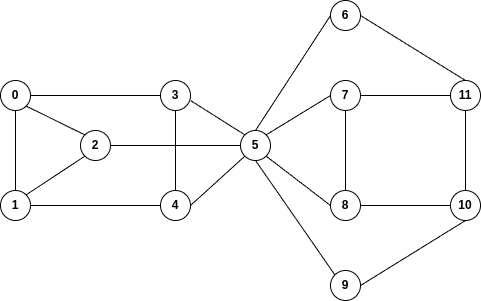
\includegraphics[width=0.4\textwidth]{pictures/ex-coloring-1.png} 
	\caption{Ένα AT-free γράφημα με 12 κόμβους}
	\label{fig:ex-coloring-1}
\end{figure}

Το γράφημα περνάει τον έλεγχο της γραμμής 1 και της γραμμής 5 αφού δεν περιέχει κάποιο $K_4$ αλλά και ούτε κάποιο διαμάντι. Ο αλγόριθμος σταματάει στην γραμμή 9 αφού στο γράφημα εντοπίζεται ένας ελάχιστος σταθερός διαχωριστής $S = \{ 10, 5\}$. Ο αλγόριθμος σύμπτυξη τις ακμές του $S$ και ο αλγόριθμος καλείται ξανά αναδρομικά στο νέο γράφημα \ref{fig:ex-coloring-2}

\begin{figure}[H]
	\centering
	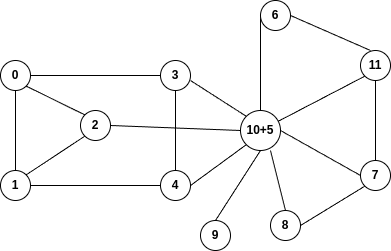
\includegraphics[width=0.4\textwidth]{pictures/ex-coloring-2.png} 
	\caption{To γράφημα μετά την σύμπτυξη των κορυφών 10,5}
	\label{fig:ex-coloring-2}
\end{figure}

Όπως είναι αντιληπτό από το παραπάνω γράφημα, από την σύμπτυξη των ακμών 10,5 το γράφημα έχει δημιουργήσει δύο διαμάντια. Στα παρακάτω δύο γραφήματα φαίνεται πως ο αλγόριθμος \ref{alg:coloring} στην γραμμή 5 εξαλείφει τα διαμάντια συμπτύσσοντας τις κορυφές $u$, $v$ για τις οποίες ισχύει $|N(u) \cap N(v)| \geq 2$.

\begin{figure}[H]
	\centering
	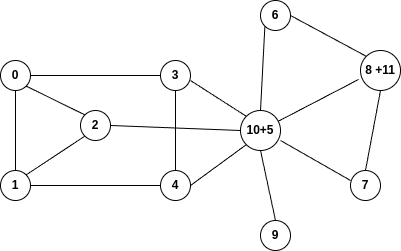
\includegraphics[width=0.4\textwidth]{pictures/ex-coloring-3.png} 
	\caption{To γράφημα μετά την σύμπτυξη των κορυφών 8,11}
	\label{fig:ex-coloring-3}
\end{figure}

\begin{figure}[H]
	\centering
	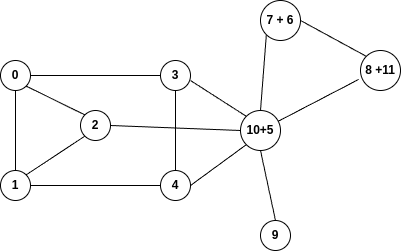
\includegraphics[width=0.4\textwidth]{pictures/ex-coloring-4.png} 
	\caption{To γράφημα μετά την σύμπτυξη των κορυφών 7,6}
	\label{fig:ex-coloring-4}
\end{figure}

Το γράφημα μετά την σύμπτυξη των ακμών 7,6 φτάνει στην γραμμή 13 του αλγορίθμου\ref{alg:coloring}. Το γράφημα για να μπορέσει να χρωματιστεί πρέπει να χωριστεί σε μπλοκς. Τα μπλοκς του γράφηματος \ref{fig:ex-coloring-4} φαίνονται στον παρακάτω πίνακα με την σειρά που θα χρωματιστούν. 

\begin{table}[H]
	\centering
	\begin{tabular}{|c|c|}
		\hline
		Μπλοκ & Κορυφές του Μπλοκ \\
		\hline
		1 & $\{1, 10+5, 2, 3, 4, 0 \}$ \\
		0 & $\{8+11, 7+6, 10+5 \}$ \\
		2 & $\{9 \}$ \\
		\hline
	\end{tabular}
	\caption{Πίνακας με τα μπλοκς του γραφήματος}
	\label{tab:blocks}
\end{table}

Χρωματίζουμε εναλλάξ τους κόμβους του κάθε μπλοκ με τα χρώματα \textcolor{red}{κόκκινο}, \textcolor{green}{πράσινο} και \textcolor{blue}{μπλε}. 

\begin{figure}[H]
	\centering
	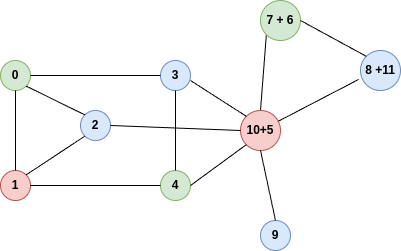
\includegraphics[width=0.4\textwidth]{pictures/ex-coloring-before-expansion.png} 
	\caption{To συμπτυγμένο" γράφημα μετά τον 3-χρωματισμό}
	\label{fig:ex-coloring-before-expansion}
\end{figure}

Από το Θεώρημα \ref{theor:1.3}, γνωρίζουμε ότι οι συμπτυγμένοι κόμβοι στο αρχικό γράφημα (βλ. Σχήμα \ref{fig:ex-coloring-1}) θα έχουν το ίδιο χρώμα. Για παράδειγμα, οι κόμβοι 10 και 5 θα είναι \textcolor{red}{κόκκινοι}.

\begin{figure}[H]
	\centering
	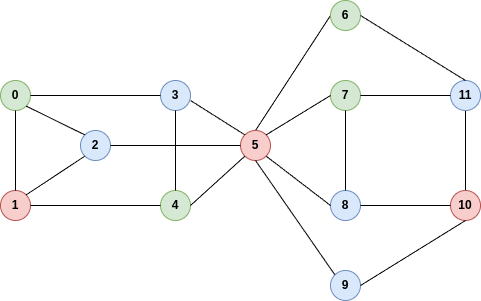
\includegraphics[width=0.8\textwidth]{pictures/ex-coloring-after-expansion.png} 
	\caption{To γράφημα μετά το τέλος του αλγορίθμου}
	\label{fig:ex-coloring-after-expansion}
\end{figure}














